\model{The Circle Class}

Unified Modeling Language (UML) provides a way of graphically illustrating a class's design, independent of the programming language.

\begin{center}
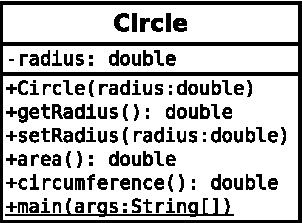
\includegraphics{Circle.pdf}
\end{center}


\quest{15 min}


\Q Consider the \java{Circle} class:

\begin{enumerate}
\item How many attributes does it have?
\ans[3em]{1}

\item How many methods does it have?
\ans[3em]{6}
\end{enumerate}


\Q Based on \ref{die-class.tex} and \ref{\currfilename}, what is typically \java{public} and what is typically \java{private}?

\begin{answer}[2em]
Methods are typically public,
and attributes are typically private.
\end{answer}


%\Q How would you declare a variable named \java{unit} that is a \java{Circle} object?
%
%\begin{answer}[1em]
%\tt Circle unit;
%\end{answer}


%\Q How would you initialize \java{unit} to be a new \java{Circle} with a radius of 1.0?
%
%\begin{answer}[1em]
%\tt unit = new Circle(1.0);
%\end{answer}


\comment{The following questions will have you implement the \java{Circle} class exactly as shown in the UML diagram above.
Do not worry about writing Javadoc comments for this activity.}


\Q Write the code that declares the \java{radius} attribute.
An outline of \textit{Circle.java} is provided below for context.

\begin{javalst}
public class Circle {
\end{javalst}

{\tt ~~~}\ans{\tt private double radius;}

\medskip

\begin{javalst}
    // constructor goes here
    
    // other methods go here
}
\end{javalst}


\Q Write the code for the \java{Circle} constructor.
Notice that, in contrast to \ref{die-class.tex}, the \java{Circle} constructor has a parameter.
Assign the parameter \java{radius} to the attribute \java{this.radius}.

\begin{answer}[5em]
\begin{javaans}
public Circle(double radius) {
    this.radius = radius;
}
\end{javaans}
\end{answer}


\Q Write the code for \java{getRadius}.
(Refer to \ref{die-class.tex} for an example.)

\begin{answer}[5em]
\begin{javaans}
public double getRadius() {
    return this.radius;
}
\end{javaans}
\end{answer}


\Q Write the code for \java{setRadius}.
Like the constructor, it should assign the parameter to the corresponding attribute.

\begin{answer}[5em]
\begin{javaans}
public void setRadius(double radius) {
    this.radius = radius;
}
\end{javaans}
\end{answer}


\Q Write the code for \java{area}.
The area of a circle is $\pi r^2$.

\begin{answer}[5em]
\begin{javaans}
public double area() {
    return Math.PI * radius * radius;
}
\end{javaans}
\end{answer}


\Q Write the code for \java{circumference}.
The circumference of a circle is $2 \pi r$.

\begin{answer}[5em]
\begin{javaans}
public double circumference() {
    return 2.0 * Math.PI * radius;
}
\end{javaans}
\end{answer}


\Q \label{circmain}
Write a \java{main} method that creates a \java{Circle} object with a radius of 2.0 and displays its area and circumference (using \java{println}).

\begin{answer}[8em]
\begin{javaans}
public static void main(String[] args) {
    Circle circle = new Circle(2);
    System.out.println(circle.area());
    System.out.println(circle.circumference());
}
\end{javaans}
\end{answer}
